\documentclass[margin=3mm]{standalone}
\usepackage{tikz}

\begin{document}
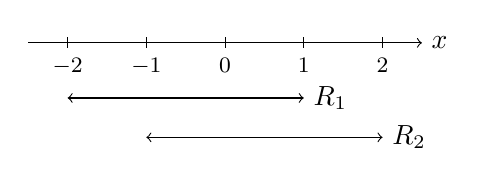
\begin{tikzpicture}
    \draw[->] (-2.5,0) -- (2.5,0) node[right] {$x$};
    \draw[distance=0.5mm,<->] (-2,-0.7) -- (1,-0.7) node[right] {$R_{1}$};
    \draw[distance=0.5mm,<->] (-1,-1.2) -- (2,-1.2) node[right] {$R_{2}$};
    \foreach \x in {-2,-1,0,1,2}
    \draw[shift={(\x,0)},color=black] (0pt,2pt) -- (0pt,-2pt) node[below] {\footnotesize $\x$};
\end{tikzpicture}

\end{document}